\chapter{Solving unseen geometric constructions}
\label{chapter_unseen_levels}
We have already mentioned, there are multiple predictions in Mask {R-CNN} models (see Section \ref{inferene_highest_score}). In this chapter, we further examine those predictions. To do so, we create a program for the exploration of hypotheses given by multiple models. Then we introduce the hypothesis tree search for solving unseen levels. Lastly, we analyze the inference of unseen levels with the leave-one-out method.
\section{Hypotheses generated by Mask {R-CNN}}
Each primary detection by the Mask {R-CNN} model described in Chapter \ref{mrcnn_chapter} can be transformed into an action. We denote each action, its arguments and results as ``hypothesis''. The result of an action contains the reward and output geometric primitive constructed during the action execution. The reward indicates whether the output primitive is a part of the goal or not. If an action constructs part of the goal, the reward is equal to $1/n$, where $n$ is the number of primitives in the goal, otherwise, it is equal to zero. In Table \ref{hypothesis_explorer_detail} in Sub-figure d) we can see a hypothesis that successfully finished one of the four goals and hence it has a reward equal to $0.25$.  We  can extract multiple actions from the Mask R-CNN model outputs and then transform them into multiple hypotheses. 
\newline \newline
When we obtain hypotheses from the Mask {R-CNN}, we can explore the construction space defined by those hypotheses. Furthermore, we can also use hypotheses from multiple models trained for different tasks. However, Mask {R-CNN} scores across hypotheses from different models are not well calibrated. For exploration purposes, we developed an interactive program where the user can choose multiple trained models and levels for inference, and then run inference where the user can choose which hypothesis should be used at a given time. In Figure \ref{hypothesis_explorer} we can see a screenshot from the program followed with hypotheses details in Table \ref{hypothesis_explorer_detail}. Hypothesis visualization is based on our Euclidea visualization (see Section \ref{euclidea_vizualization}) with the addition of the hypothesis result object to the blue channel. The program can get hypotheses from any model, but in this thesis, we prepared models trained on the first 6 Euclidea level packs:
\begin{itemize}
\item 68 ``level'' models (one for each level). 
\item 6 ``level-pack'' models (one for each level pack).
\item 1 ``all'' model (for level packs Alpha - Zeta).
\end{itemize}

\begin{figure}[h!]
\centering
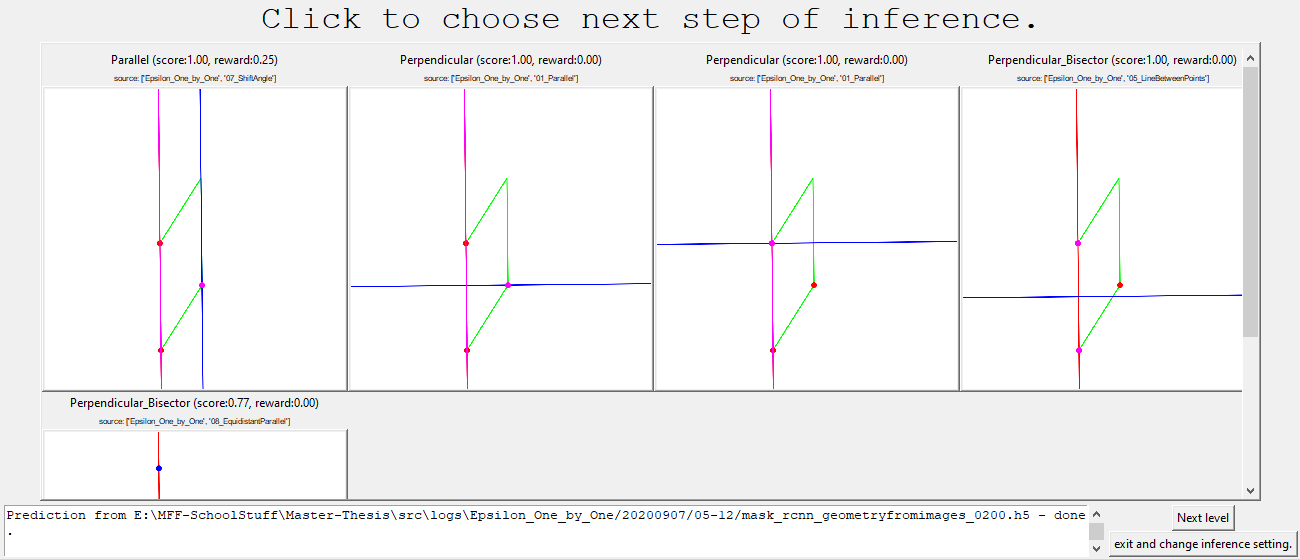
\includegraphics[width=140mm]{img/hypothesis_explorer/explorer.png}
\caption{Screenshot of our hypothesis explorer program. Construction of the level \textit{Epsilon 03}, Parallelogram given by 3 points. To solve this level, we have all level-specific models for Epsilon, with the exception of the model for \textit{Epsilon 03}. In this step of construction, we have 5 different hypotheses given by 4 models. Other models either do not give any hypotheses or give hypotheses that can be grouped with other hypothesis (see Section \ref{reducing_hypotheses}), we consider only a single hypothesis per group. In the program, the user chooses manually which hypothesis should be constructed. Details of each hypothesis are in Table \ref{hypothesis_explorer_detail} }
\label{hypothesis_explorer}
\end{figure}

\begin{longtable}{m{0.5\textwidth}m{0.5\textwidth}}
         \begin{subfigure}
         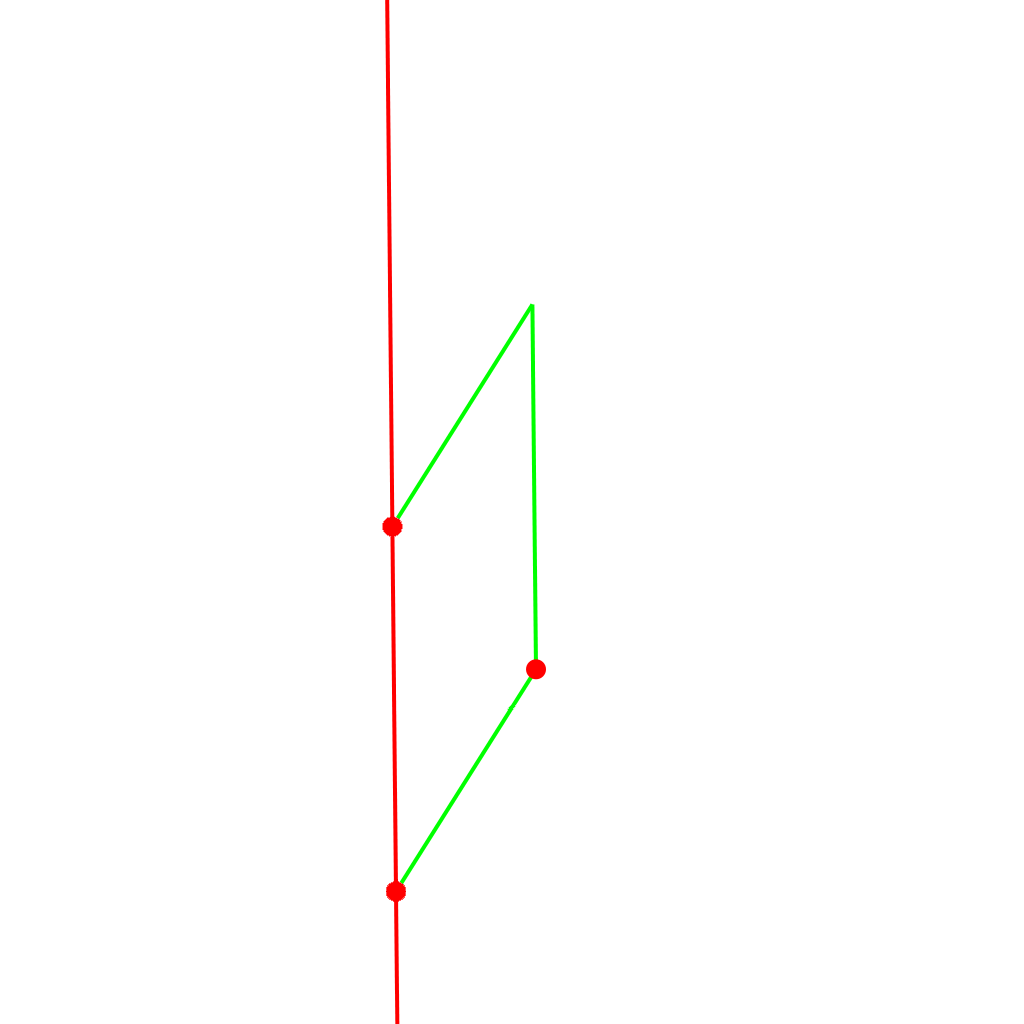
\includegraphics[width=70mm]{img/hypothesis_explorer/input.png}
         \label{xx}
         \end{subfigure}
         &
         \begin{subfigure}
         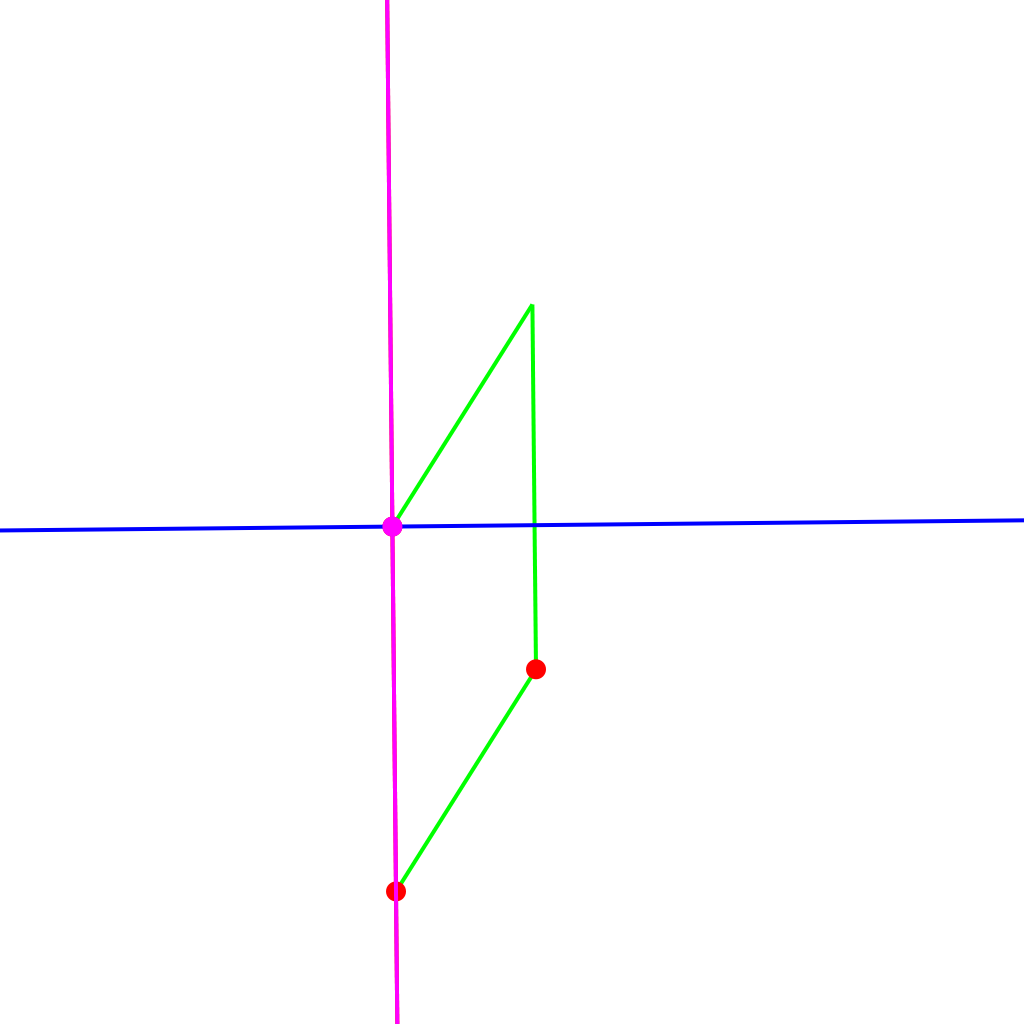
\includegraphics[width=70mm]{img/hypothesis_explorer/source_01_score_0.999_Perp.png}
         \label{xx}
         \end{subfigure}
         \\
         a) The Current state without any hypothesis, Input for the Mask {R-CNN} models. &
         b) source: Epsilon 01, score: 0.99, tool: Perpendicular, reward: 0.0 \\
         \begin{subfigure}
         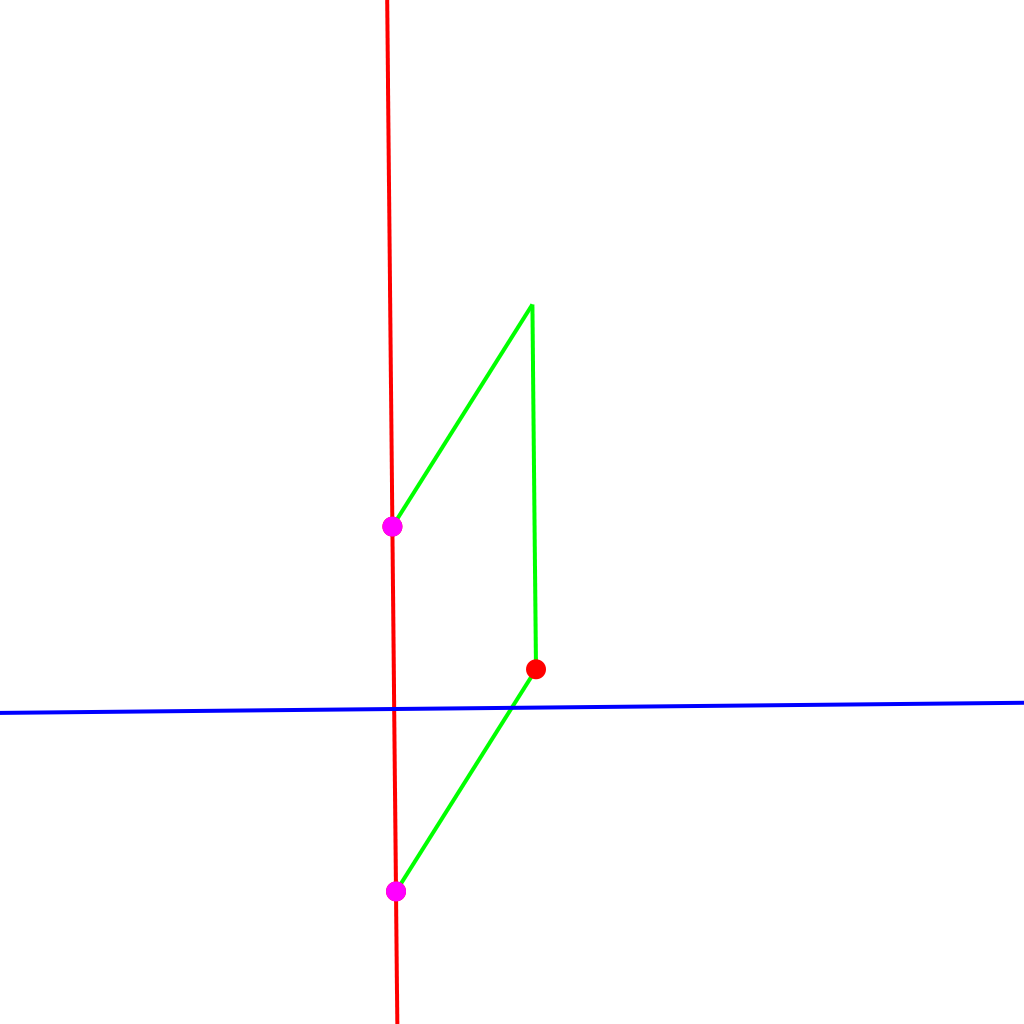
\includegraphics[width=70mm]{img/hypothesis_explorer/source_05_score_0.996_PerpBisector.png}
         \end{subfigure}
         &
         \begin{subfigure}
         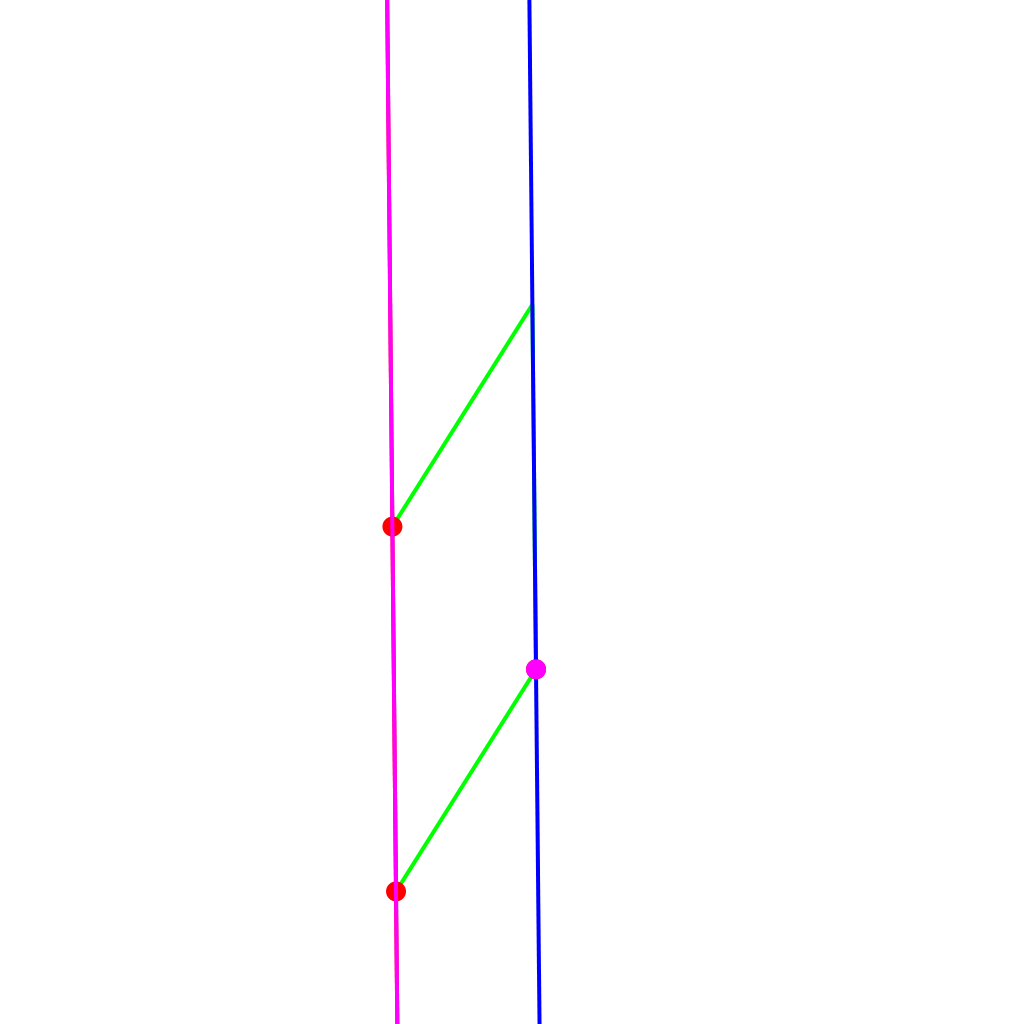
\includegraphics[width=70mm]{img/hypothesis_explorer/source_07_score_0.999_Parallel.png}
         \end{subfigure}
         \\
          c) source: Epsilon 05, score: 0.99, tool: Perpendicular Bisector, reward: 0.0 &
         d) source: Epsilon 07, score: 0.99, tool: Parallel line, reward: 0.25\\
         \begin{subfigure}
         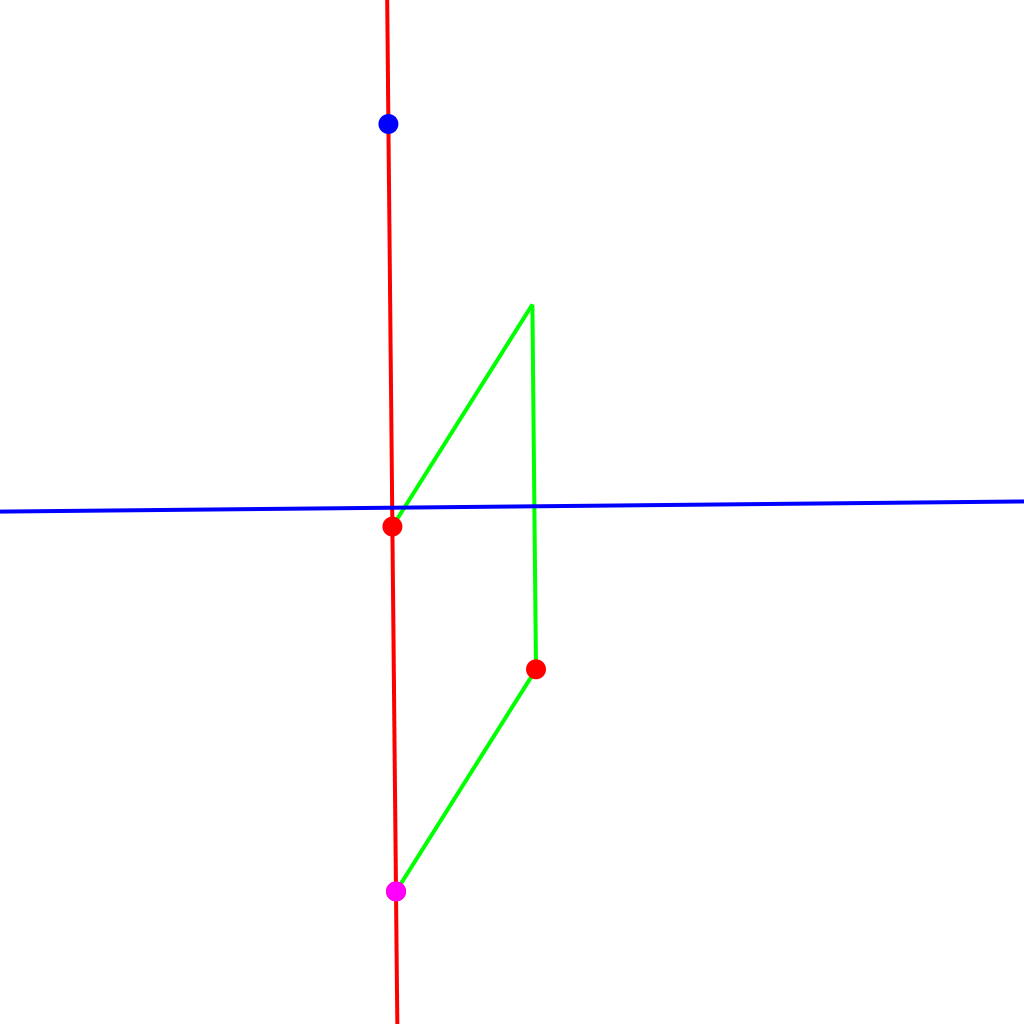
\includegraphics[width=70mm]{img/hypothesis_explorer/source_08_score_0.77_PerpBisector.png}
         \end{subfigure}
         &
         \begin{subfigure}
         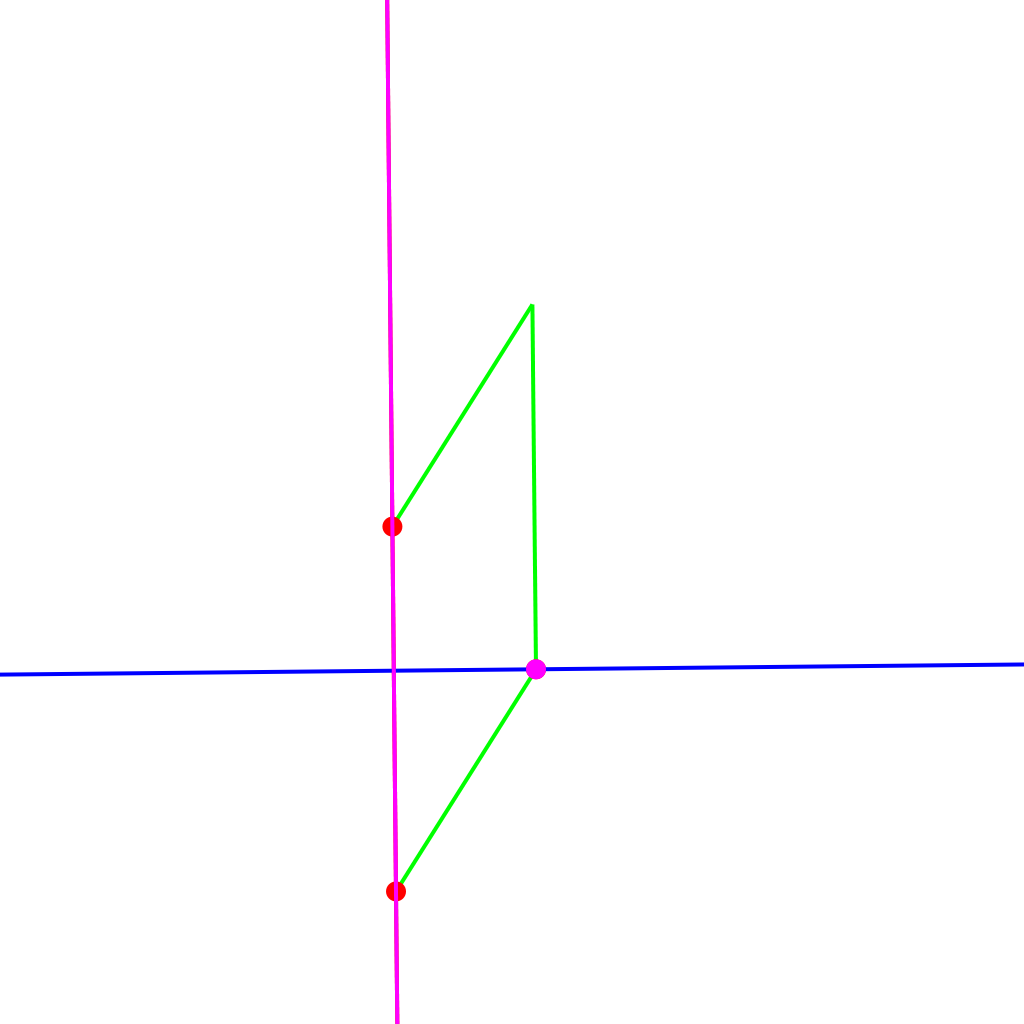
\includegraphics[width=70mm]{img/hypothesis_explorer/source_01_score_0.999_Perpl.png}
         \end{subfigure}
         \\
         e) source: Epsilon 08, score 0.77, tool: Perpendicular Bisector, reward: 0.0 &
         f) source: Epsilon 01, score: 0.99, tool: Perpendicular, reward: 0.0 
         \\
\caption{Five different hypotheses for solving the level \textit{Epsilon 03}. This table is a detail for Figure \ref{hypothesis_explorer}. Thus each hypothesis corresponds to its miniature in Figure \ref{hypothesis_explorer}. Each figure contains the current state (red), remaining goal (green), hypothesis produced by Mask R-CNN (blue), and highlighted arguments of the tool (purple). We can see that hypothesis d) has a reward equal to $0.25$. Hence d) is a correct step that should be picked in this step.}
\label{hypothesis_explorer_detail}
\end{longtable}

\section{Inference with tree search}
\label{hypotheses_tree_search}
In the previous section, we described how to get hypotheses from multiple Mask {R-CNN} models. Now we will search for the target construction within these hypotheses. To compare the results of the hypothesis tree search with the exhaustive tree search from Chapter \ref{chapter_exhaustive_search}, we use iterative deepening. The tree search has to build an input image and run predictions of all Mask {R-CNN} models in each node, which significantly increases the time spent on one node. However, the hypothesis tree search should have a significantly lower branching factor.

\section{Reducing the number of hypotheses}
\label{reducing_hypotheses}
Hypotheses produced by different models increase the branching factor and thus also the search time. In order to speed up the tree search, we group similar hypotheses and explore only one of them. We consider two hypotheses to be similar if they have the same output geometric primitive. Note that they can have different arguments, including different tools.

\section{Cheat moves}
In Euclidea, a goal cannot be finished by simply drawing a similar line or circle (see Section \ref{about_euclidea}). We denote those as cheat moves. However, a hypothesis given by the models may suggest drawing a cheat move. We can recognize some hypothesis of a cheat move by coordinates of its arguments. One of its arguments is a point in space without any geometric primitive nearby. Note that with the mentioned approach, we cannot find every cheat move. Some levels aim to find a specific point on the line or circle, which can be guessed instead of constructed. Cheat move hypotheses can be removed as they do not lead to the goal. However, when all necessary points are constructed further in construction, this cheat move prediction becomes a legitimate move.

\section{Leave-one-out evaluation}
\label{leave_one_out_method}
We use the ``leave-one-out'' method to evaluate performance on unseen levels. For our purposes the method inputs are levels with corresponding level specific models. To evaluate accuracy of a level we use all other models, e.g.~models that were not trained for this level. We can also apply this on whole level pack models. Note that we should avoid a situation where 2 different models are trained for the same task, for example we should not have models for \textit{Alpha 01} level and Alpha level pack, since both models are trained for \textit{Alpha 01}. For the inference we use the hypothesis tree search (see Section \ref{hypotheses_tree_search}).
Note that due to score miss calibration, the top score detection (see Section \ref{top_score_inference}) approach cannot be used when we have multiple models. The accuracy of the leave-one-out set-up is reported in the experimental Section \ref{eval_of_unseen_levels}.

\section{Connections between levels}
\label{connections}
When evaluating a level using leave-one-one method, we might use hypotheses only from a fraction of level specific models. We denote that level $X$ is ``connected'' to level $Y$, when a model trained for $Y$ contributes to a successful construction with any hypothesis during the inference for level $X$. Note that relation ``connected'' is not reflexive, e.g.~ when $X$ is connected to $Y$, then $Y$ is not necessary connected to $X$. Since we run hypothesis tree search during the leave-one-out evaluation, we obtain connections in following way: If the search is successful, we collect models that contributed to the solution in the final backtracking of the search.


